\section{Transport Layer}
\paragraph{Schicht 4: Transportschicht}

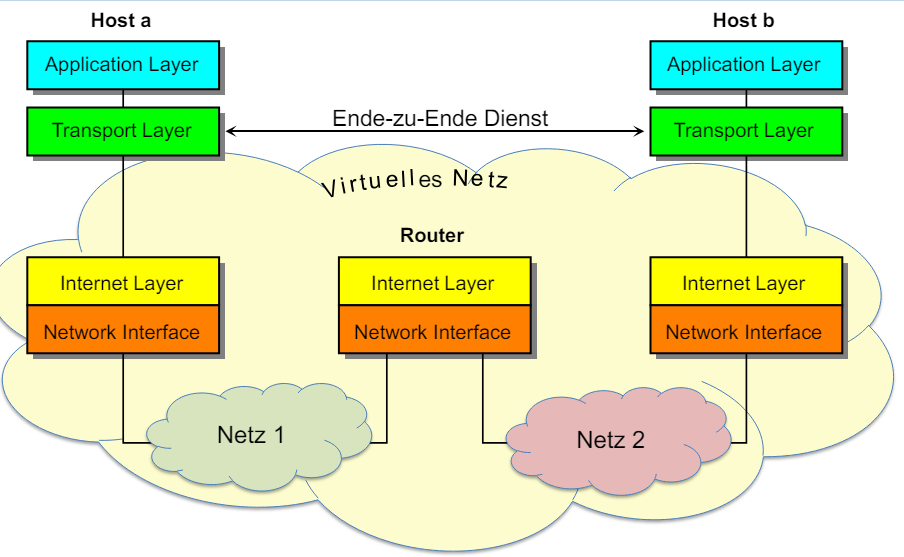
\includegraphics[width=0.75\linewidth]{images/transportlayer.png}

\begin{definition}{Transportlayer}\\
    Der Transport Layer bildet auch die Schnittstelle zwischen dem Betriebssystem (Kernel Space) und den Anwendungen (User Space)\\
    Der Zugriff auf die Funktionen des Transport Layers erfolgt via einer klar definierten Schnittstelle (Sockets)
\end{definition}

\begin{definition}{Kapselung}
    \begin{itemize}
        \item Die Applikationsdaten werden von den Protokollen des Transport Layers in ein IP-Paket gekapselt
        \item Das gekapselte Protokoll wird im IP-Header im Feld Protocol angegeben
        \item Das "Protocol" Feld unterscheidet UDP und TCP Daten
    \end{itemize}
\end{definition}

\begin{concept}{Adressierung der Applikation durch Port Nummern}\\
    Der Client adressiert mit der Destination Port Nummer die gewünschten Server-Applikation
    \begin{itemize}
        \item sonst weiss das TCP/UDP-Modul im Empfänger nicht, welche Applikation gemeint ist
        \item für die Source Port Nummer verwendet der Client (meist) eine zufällige Port Nummer im Bereich >1'023 (wird vom Betriebssystem vergeben)
    \end{itemize}
\end{concept}

\subsubsection{UDP - User Datagram Protocol}

\begin{definition}{UDP}
    dient dem Multi- und Demultiplexen der Datagramme zu den Applikationen.
    \begin{itemize}
        \item Verbindungslos
        \item Unzuverlässig
    \end{itemize}
\end{definition}

\begin{concept}{UDP-Header}
    \begin{itemize}
        \item \textcolor{green}{Source Port} Sendende Applikation
        \item \textcolor{green}{Destination Port} Applikation des Empfängers
        \item \textcolor{blue}{Message Length} Länge des Datagramms
        \item \textcolor{purple}{Checksum} Prüfsumme über einen Pseudo-Header, UDP-Header und Daten
        \begin{itemize}
            \item kann Null sein
            \item Pseudo-Header: IP Source- und Destination Address, Protocol Feld, Länge des Datagramms
            \begin{itemize}
                \item so können fehlgeleitete Datagramme erkannt werden
                \item z.B. aufgrund eines Bit-Flip
            \end{itemize}
        \end{itemize}
    \end{itemize}
        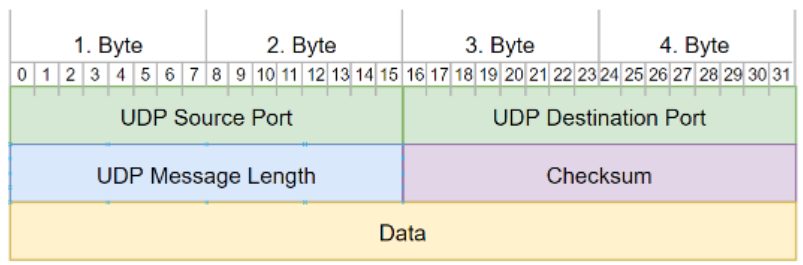
\includegraphics[width=1\linewidth]{images/udp.png}
\end{concept}

\begin{concept}{Adressierung und Multiplexing}\\
        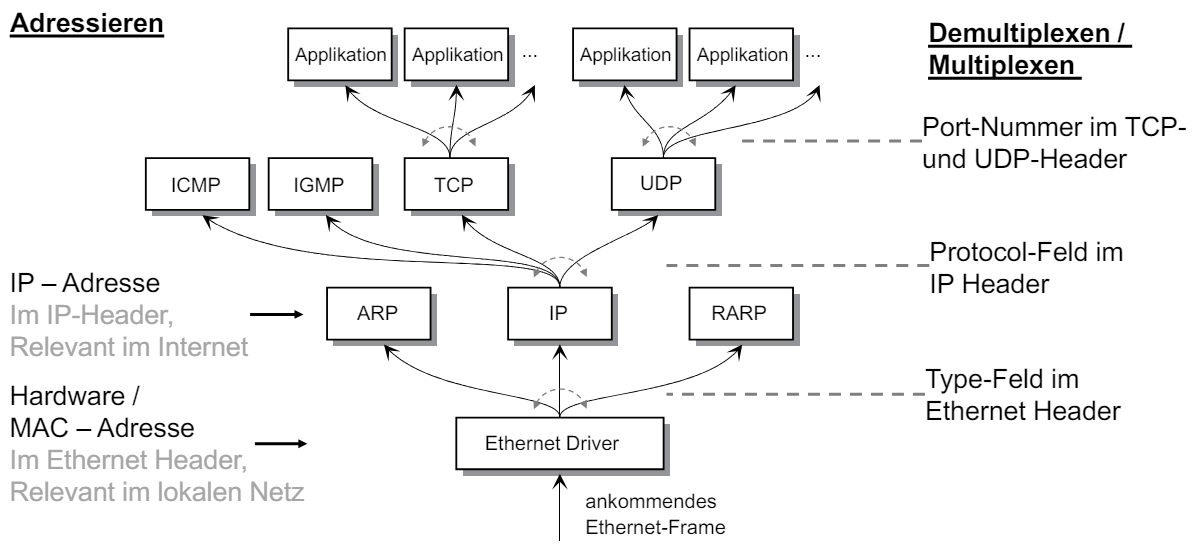
\includegraphics[width=1\linewidth]{images/adress_multiplex.png}
\end{concept}

\begin{formula}{Port-Nummern}
    \begin{itemize}
        \item \textcolor{green}{System Ports (Well-Known)} Feste Port-Nummern, für bekannte Appl. reserviert
        \item \textcolor{blue}{User Ports (Registered)} Reservierter Bereich für herstellerspezifische Appl.
        \item \textcolor{yellow}{Dynamic / Private Ports} Frei verfügbare Ports
    \end{itemize}
        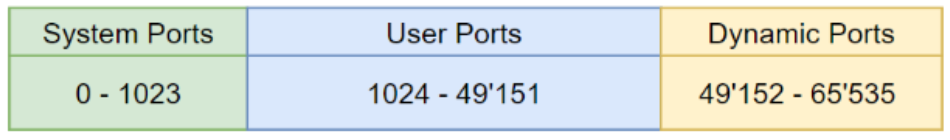
\includegraphics[width=1\linewidth]{images/portnummern.png}
\end{formula}

\subsection{TCP - Transmission Control Protocol}

\begin{definition}{TCP} Eigenschaften
    \begin{itemize}
        \item Verbindungsorientierte Übertragung: Zuerst wird eine Verbindung zwischen Client- und Serveranwendung aufgebaut
        \item Zuverlässiger Verbindungsaufbau: Bevor eine TCP-Verbindung steht, muss dies von beiden Endpunkten aktiv bestätigt werden
        \item Hohe Zuverlässigkeit: Die Daten kommen ohne Datenverlust und in der richtigen Reihenfolge auf der anderen Seite an
        \item Vollduplexübertragung: Gleichzeitige, voneinander unabhängige, Übertragung in beiden Richtungen möglich
        \item Stream-Schnittstelle: Die Anwendung sendet/empfängt eine unstrukturierte Byte-Folge
        \item Graceful Termination (Verbindungsabbau): TCP gewährt die Zustellung aller Daten auch beim Verbindungsabbau
        \item Punkt-zu-Punkt Kommunikation: Zwei Applikationen tauschen Daten aus. Konzepte wie Multicast oder Broadcast existieren nicht.
    \end{itemize}
\end{definition}

\begin{definition}{Zuverlässigkeit}\\
    TCP muss diverse Probleme lösen:
    \begin{itemize}
        \item Eine Verbindung soll zuverlässig auf- und abgebaut werden können\\
        → Verbindungsaufbau, Verbindungsabbau
        \item TCP-Nachrichten können verloren, verfälscht, dupliziert und deren Reihenfolge vertauscht werden – trotzdem sollen alle Daten korrekt, vollständig und in der richtigen Reihenfolge auf der anderen Seite an die Applikation weitergegeben werden\\
        → Sequenznummern, Adaptiver Timeout, Sliding Window Protokoll
        \item Der Empfänger soll nicht mit Daten überschwemmt werden, d.h. der Sender soll sich an die Möglichkeiten des Empfängers anpassen\\
        → Flow Control mit Advertized Window Size
        \item Das Netz dazwischen soll nicht überlastet werden, damit ein vernünftiger Durchsatz für alle möglich ist\\
        → Congestion Control mit Slow Start Algorithmus
    \end{itemize}
\end{definition}

\begin{concept}{Verbindungsorientierte Kommunikation}\\
    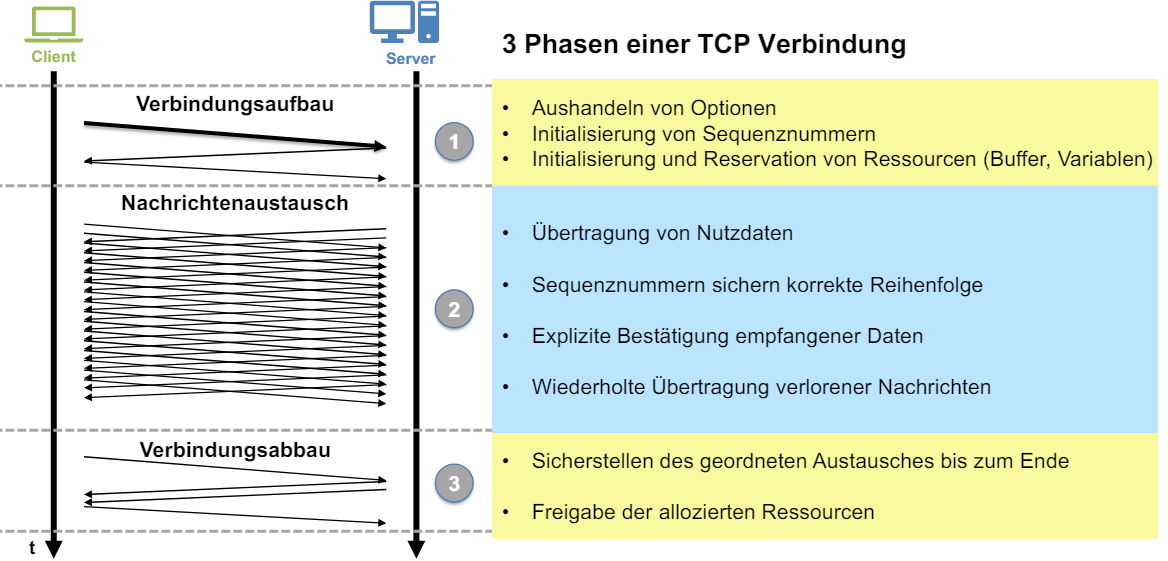
\includegraphics[width=1\linewidth]{images/verbindungsorientierte_kommunikation.png}
\end{concept}

\subsubsection{TCP Header}

\begin{definition}{Header Specs}
    \begin{itemize}
        \item TCP Header Länge: Mindestens 20 Bytes plus mögliche Optionen (+ max. 40 Bytes)
        \item Eine TCP-Verbindung besteht aus je einem Datenstrom in jeder Richtung
        \item Header beinhaltet Information für die "Vorwärtsrichtung" (Sequenznummer etc.) und für die "Rückwärtsrichtung" (Acknowledgement Nummer, Window)
    \end{itemize}
\end{definition}

\begin{concept}{TCP-Header Format}
    \begin{itemize}
        \item \textcolor{yellow}{Sequence-Nr.} Nummer zur Ordnung der Segmente
        \item \textcolor{yellow}{Acknowledgement-Nr.} n + 1 → Daten bis und mit n korrekt und vollständig angekommen
        \item \textcolor{purple}{Data Offset} Gibt an wo Daten beginnen / enden
        \item \textcolor{purple}{ECN-Flags} Explicit Congestion Notification
        \begin{itemize}
            \item Bit 8: CWR (Congestion Window Reduced)
            \item Bit 9: ECE (ECN-Echo)
        \end{itemize}
        \item \textcolor{purple}{Control Bits} Verbindungsauf- und -abbau (Bits 10-15)
        URG: Urgent Pointer
        ACK: Acknowledgement Number
        PSH: Push (sofort ohne buffern weiterleiten)
        RST: Reset (Verbindung zurücksetzen oder geschlossenen Port signalisieren)
        SYN: Synchronize (Verbindung aufbauen)
        FIN: Verbindung abbauen
        \item \textcolor{blue}{Window} Verfügbare Puffergrösse (so viele Bytes dürfen noch gesendet werden)
        \item \textcolor{purple}{Urgent Pointer} URG = 1 → Position der wichtigen Daten
        \item \textcolor{purple}{Options} Häufigste Verwendung: MSS (Maximum Segment Size) die empfangen werden kann
    \end{itemize}
    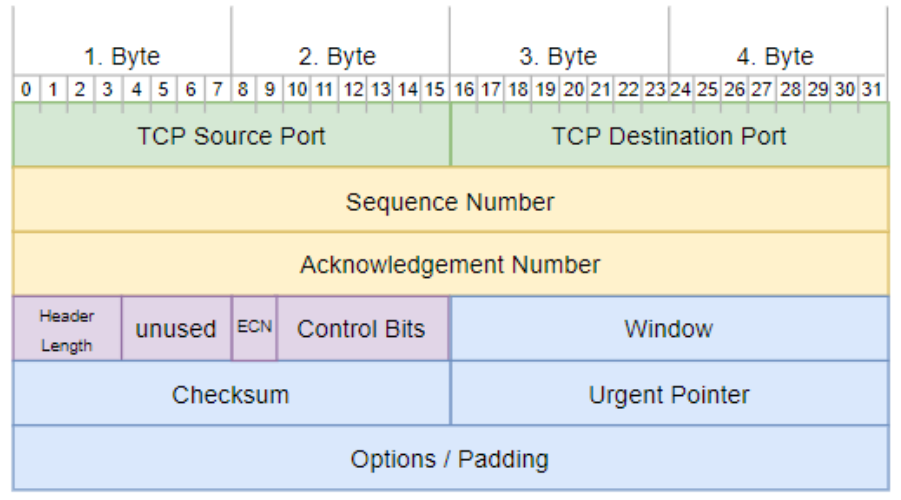
\includegraphics[width=1\linewidth]{images/tcpheader.png}
\end{concept}

\subsubsection{TCP Verkehrssteuerung}

\begin{concept}{Nachrichtenaustausch}\\
    Unabhängig für jede Richtung:
    \begin{itemize}
        \item Sequence Numbers identifizieren jedes Byte des gesendeten Nutzdatenstroms
        \begin{itemize}
            \item Sicherstellen der richtigen Reihenfolge der Daten
            \item Erkennen verloren gegangener Daten
        \end{itemize}
        \item Acknowledge Numbers identifizieren korrekt empfangene Bytes (der Gegenrichtung)
        \begin{itemize}
            \item Bestätigung korrekt empfangener Daten
            \item Erkennen verloren gegangener Daten
        \end{itemize}
        \item Flags steuern Verbindungsauf- und -abbau, signalisieren Gültigkeit von Informationen im Header und besondere Situationen.
        \begin{itemize}
            \item SYN/FIN: Verbindungsauf- und -abbau
            \item ACK: Acknowledge Number im empfangenen Segment ist gültig
            \item PSH: Daten sollen schnellstmöglich an Applikation weitergegeben werden
        \end{itemize}
    \end{itemize}
\end{concept}

\begin{definition}{Zustände}
    \begin{itemize}
        \item \textcolor{yellow}{LISTEN} Auf Anforderung warten
        \item \textcolor{yellow}{SYN-SENT} Anforderung geschickt
        \item \textcolor{yellow}{SYN-RECEIVED} Anforderung erhalten
        \item \textcolor{green}{ESTABLISHED} Verbindung besteht
        \item \textcolor{yellow}{FIN-WAIT-1} Abbauanforderung geschickt
        \item \textcolor{yellow}{FIN-WAIT-2} Abbauanforderung bestätigt
        \item \textcolor{yellow}{CLOSE-WAIT} Auf Lokale Verbindung warten
        \item \textcolor{yellow}{LAST-ACK} Verbindungsabbau bestätigt
        \item \textcolor{yellow}{TIME-WAIT} Letzte Bestätigung gesendet
    \end{itemize}
\end{definition}

\begin{KR}{Verbindungsaufbau}\\
        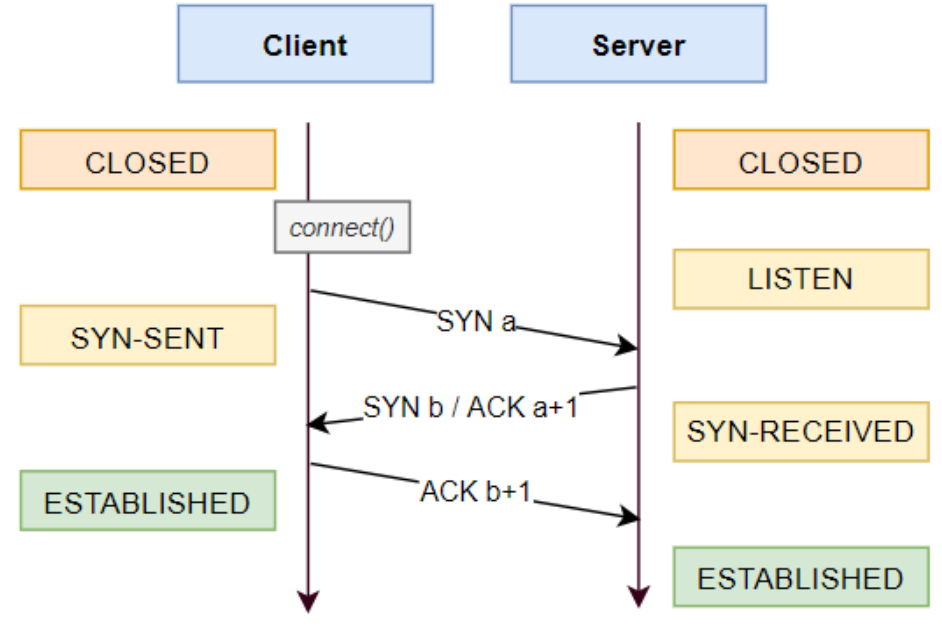
\includegraphics[width=1\linewidth]{images/verbindungsaufbau.png}
\end{KR}

\begin{KR}{Datenaustausch}\\
        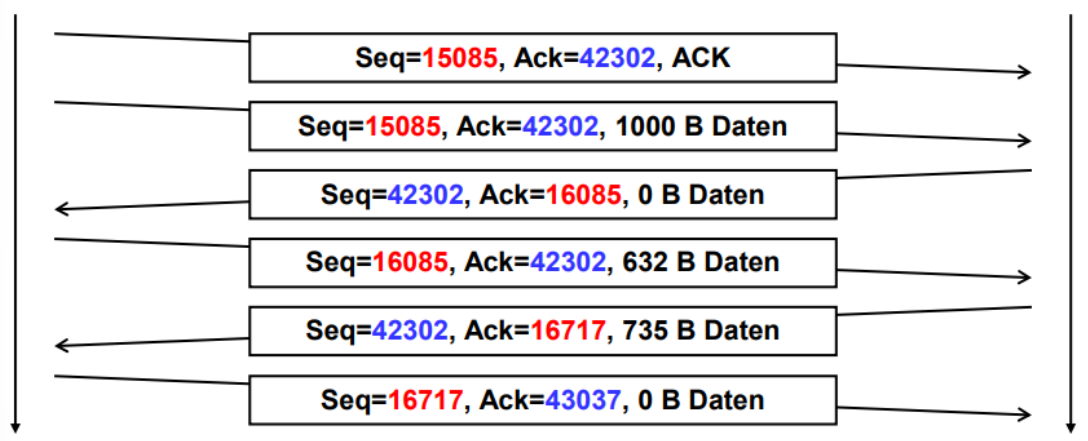
\includegraphics[width=1\linewidth]{images/datenaustausch.png}
\end{KR}

\begin{KR}{Verbindungsabbau}\\
        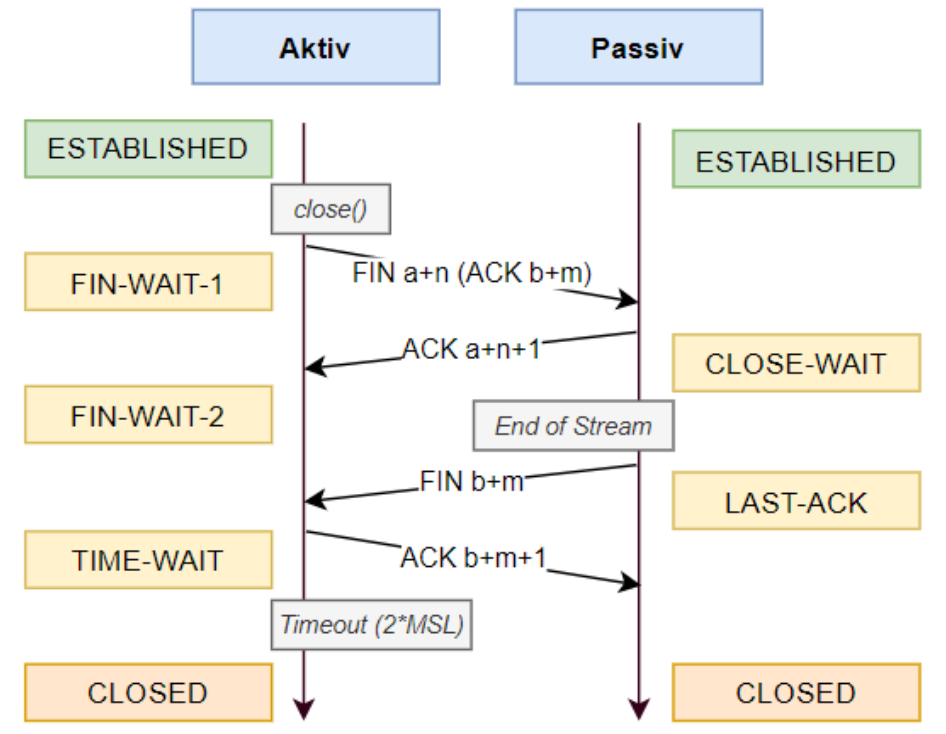
\includegraphics[width=1\linewidth]{images/Verbindungsabbau.png}
\end{KR}

\begin{example}
    Verbindungsaufbau:
    \begin{itemize}
        \item Server „horcht“ (LISTEN) auf einer bestimmten Port Nummer (z.B. 80 für einen HTTP Server)
        \item Client sendet Segment mit SYN=1 und zufälliger initialer Sequenznummer a (z. Bsp. 15'000) (ACK=0, weil Acknowledgement Nummer ungültig)
        \item Server bestätigt Sequenznummer mit Acknowledement Nummer a+1 (15'001) und ACK=1 und wählt zufällige initiale Sequenznummer b (z. Bsp. 42'300) und setzt SYN=1
        \item Client bestätigt b mit Acknowledement Nummer b+1 (42'301)
        \begin{itemize}
            \item Erstes Byte vom Client zum Server hat Sequenznummer a+1
            \item Erstes Byte vom Server zum Client hat Sequenznummer b+1
        \end{itemize}
    \end{itemize}
        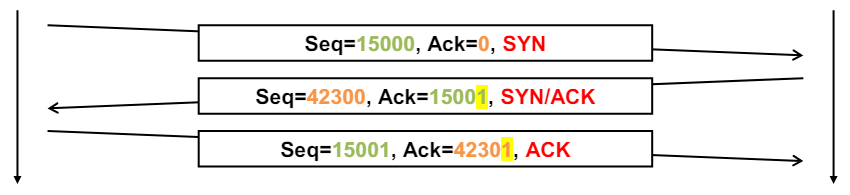
\includegraphics[width=0.75\linewidth]{images/example_verbindungsaufbau_tcp.png}
\end{example}

\begin{example}
    Während des Datenaustausches werden TCP-Nachrichten bi-direktional ausgetauscht
    \begin{itemize}
        \item Sequenznummer: Position des ersten Bytes der Daten im gesamten TCP-Datenstrom
        \item Acknowledgement Nummer: Sequenznummer des nächsten erwarteten Bytes
        \item ACK Flag: immer gesetzt
    \end{itemize}
        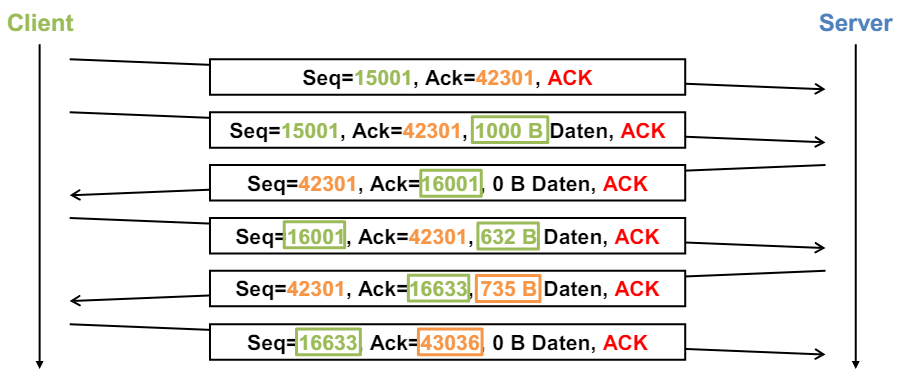
\includegraphics[width=0.75\linewidth]{images/tcp_datenaustausch_ex.png}
\end{example}

\begin{example}
    Beide Seiten können den Verbindungsabbau einleiten
    \begin{itemize}
        \item Ist eine Richtung geschlossen (FIN, ACK), so können in die andere Richtung immer noch Daten gesendet werden; dieser Verbindungszustand wird als Half-Closed bezeichnet.
        \begin{itemize}
            \item In Richtung der "geschlossenen" Verbindung wird nicht mehr kommuniziert (Acknowledge number mismatch)
        \end{itemize}
        \item Falls die zweite Seite die Verbindung auch schliesst, können die 3. und die 4. Nachricht zusammengefasst werden → FIN/ACK
    \end{itemize}
        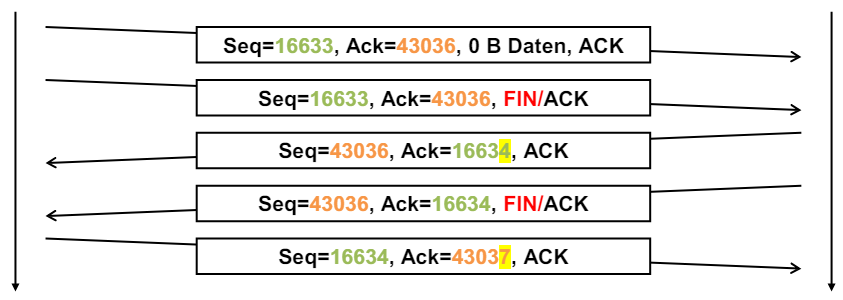
\includegraphics[width=0.75\linewidth]{images/tcp_verbindungsabbau_ex.png}
\end{example}

\begin{concept}{Zustandsdiagramm}\\
    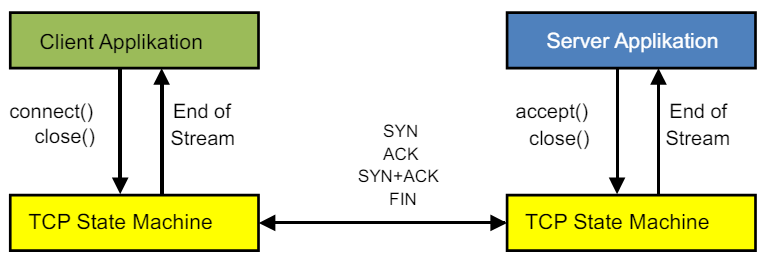
\includegraphics[width=0.5\linewidth]{images/short_overview_zustandsdiagramm.png}
    \begin{itemize}
        \item Um die verschiedenen Zustände zu durchlaufen, existiert beim Client und Server pro Verbindung je eine TCP State Machine
        \item Applikationen beeinflussen die TCP State Machines mit Systembefehlen
        \begin{itemize}
            \item listen(), connect(), close()
        \end{itemize}
        \item Die TCP State Machines signalisieren sich Events mit speziellen Flags der Control Bits im TCP-Header einer TCP-Nachricht:
        \begin{itemize}
            \item SYN, ACK, FIN
        \end{itemize}
    \end{itemize}
    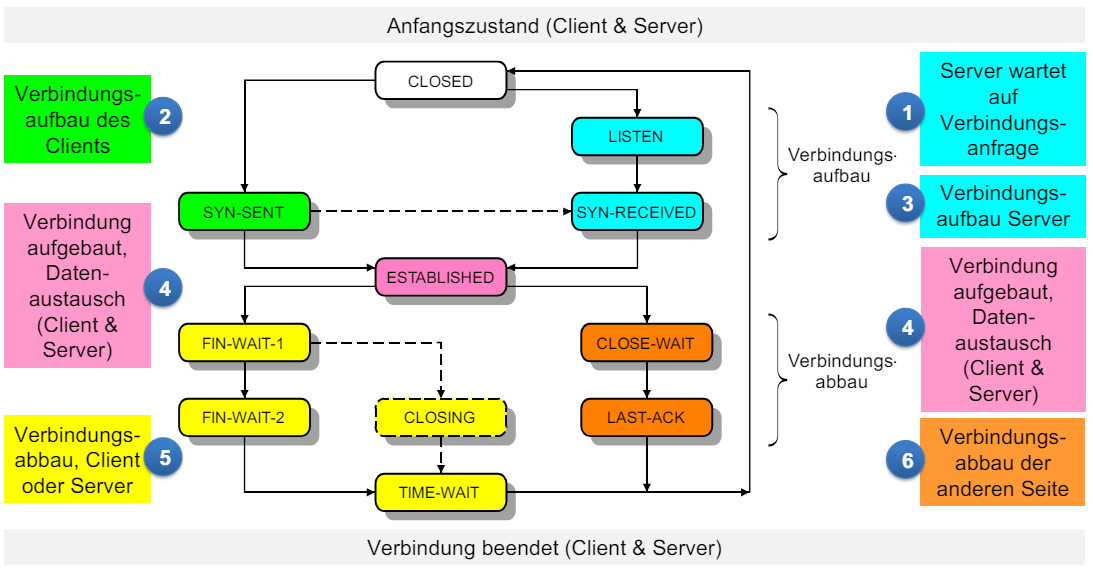
\includegraphics[width=1\linewidth]{images/zustandsdiagramm_tcp.png}
\end{concept}

\begin{example2}{Datenaustausch}\\
    Geben Sie die Seq- und Ack-Nummern der Meldung M (1000 Bytes von Client zum Server) an und zeichnen Sie die entsprechenden Positionen ein. Beachten Sie, dass 1000 Bytes vom Server noch nicht vom Client empfangen wurden.\\
    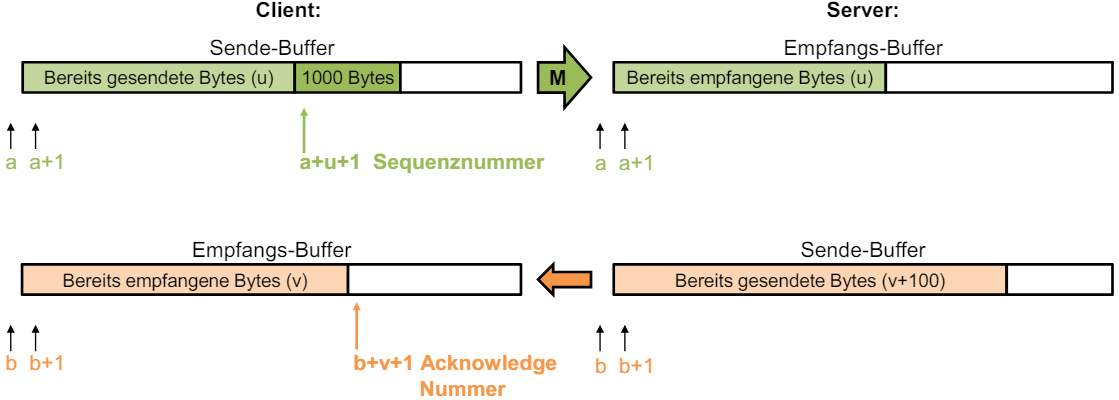
\includegraphics[width=1\linewidth]{images/datenaustausch_tcp_example.png}
\end{example2}

\subsubsection{TCP Adaptive Elemente}

\begin{definition}{Umgang mit dynamischen Situationen}
    \begin{itemize}
        \item Erkennung von verlorenen Telegrammen (Round Trip Time)
        \begin{itemize}
            \item Kann je nach Auslastung des Netzes stark variieren
            \item Wie soll der Timeout für die Detektion von Nachrichtenverlust gewählt werden?
        \end{itemize}
        \item Überlast des Empfängers (Fluss-Steuerung, Flow Control)
        \begin{itemize}
            \item Der Empfänger erhält u.U. von Hunderten oder Tausenden von Clients Daten geschickt.
            \item Wie kann der Empfänger den Sender "steuern"?
        \end{itemize}
        \item Überlast des Netzes (Überlast-Steuerung, Congestion Control)
        \begin{itemize}
            \item Selbst wenn der Empfänger ausreichend Performance und Puffer zur Verfügung hat, kann das Netz durch "Querverkehr" überlastet werden.
            \item Wie kann der Sender das erkennen und das Netz schützen?
        \end{itemize}
    \end{itemize}
\end{definition}

\begin{concept}{Erkennung verlorener Nachrichten (Stop and Wait)}\\
    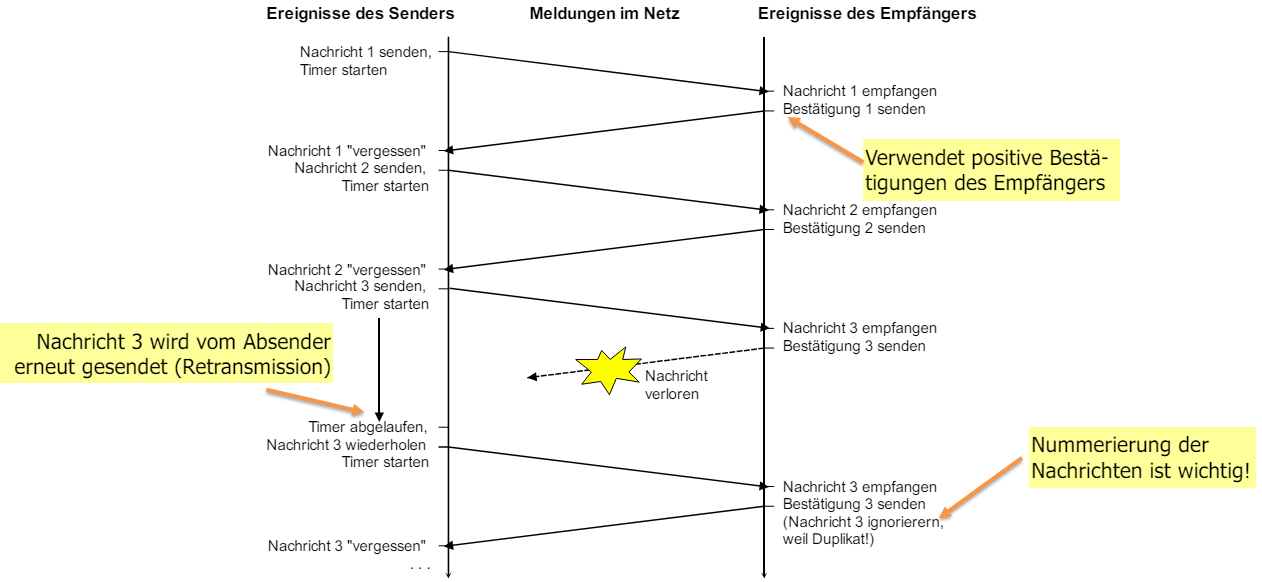
\includegraphics[width=1\linewidth]{images/erkennung_verlorener_nachrichten.png}   
\end{concept}

\begin{formula}{Round Trip Time}
    Erkennung von verlorengegangenen Telegrammen\\
    Um Fehler Paketverluste und andere Fehler zu verhindern, werden Pakete nach einer bestimmten Zeit erneut übertragen, wenn keine Bestätigung gesendet wurde. Um diese Zeit zu optimieren, misst TCP bei jeder aktiven Verbindung die \textcolor{green}{Round-Trip Time (RTT)}.
    \vspace{1mm}
    \begin{itemize}
        \item Gewichteter Mittelwert \textcolor{blue}{SRTT (Smoothed Round-Trip Time)}
    \end{itemize}
    $$\alpha = 0.125: \textcolor{blue}{SRTT_n} = (1 - \alpha) \cdot \textcolor{blue}{SRTT_{n-1}} + \alpha \cdot \textcolor{green}{RTT_n}$$
    \begin{itemize}
        \item Streuung \textcolor{yellow}{RTTVAR} des \textcolor{blue}{SRTT} der Abweichungen
    \end{itemize}
    $$\beta = 0.25: \textcolor{yellow}{RTTVAR_n} = (1 - \beta) \cdot \textcolor{yellow}{RTTVAR_{n-1}} + \beta \cdot \textcolor{blue}{SRTT_n} - \textcolor{green}{RTT_n}|$$
    \begin{itemize}
        \item Retransmission Time-Out RTO
    \end{itemize}
    $$RTO_n = \textcolor{blue}{SRTT_n} + 4 \cdot \textcolor{yellow}{RTTVAR_n}$$
\end{formula}

\begin{concept}{Fluss-Steuerung}
    Überlast des Empfängers\\
    Problem: Der Sender sendet Daten schneller, als diese vom Empfänger verarbeitet werden können. Folgen:
    \begin{itemize}
        \item Überlauf im Empfangsbuffer
        \item Daten im Empfänger gehen verloren
    \end{itemize}
    
    TCP verwendet den Sliding-Window Mechanismus um Kanalauslastung zu erhöhen. Beide Seiten einen Buffer (Window).\\
        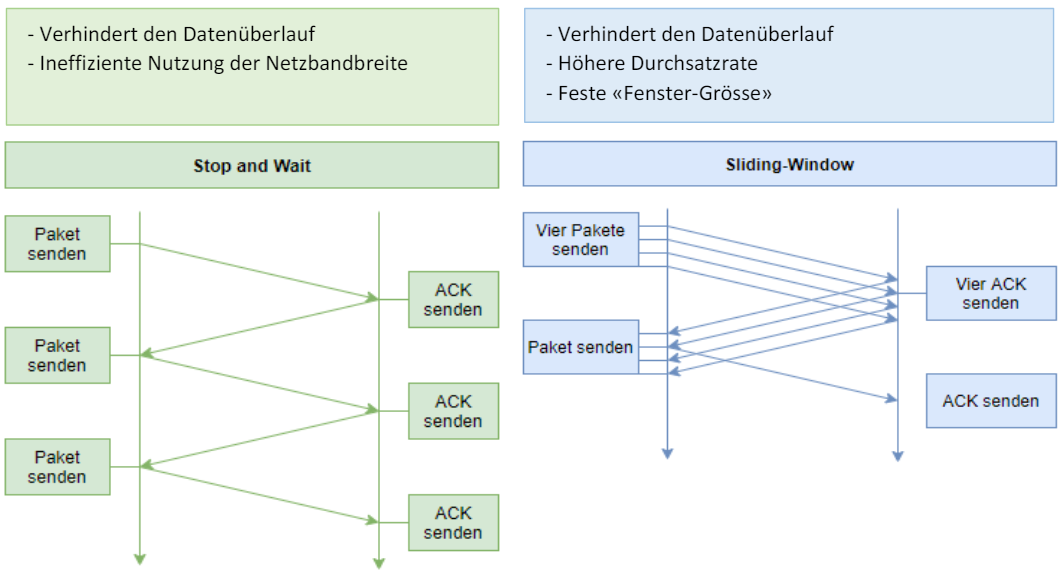
\includegraphics[width=1\linewidth]{images/fluss-steuerung.png}
\end{concept}

\begin{KR}{Sliding-Window TCP}
    \begin{itemize}
        \item Beide Richtungen arbeiten unabhängig voneinander
        \item Fenstergrösse wird in Anzahl Bytes angegeben
        \item Verbindungsaufbau: Initiale Fenstergrösse wird der anderen Seite mitgeteilt
        \begin{itemize}
            \item Typische Werte: 16 / 32 / 64 KB
        \end{itemize}
        \item Pufferplatz im Empfänger wird alloziert (der Empfänger wählt selbst die Fenstergrösse!)
        \item Mit jedem ACK wird der verfügbare Pufferplatz (in Bytes) mitgeteilt und damit die Fenstergrösse dynamisch angepasst
        \item Erhält ein Sender ein Fenstergrösse von 0 Bytes mitgeteilt, dürfen keine weiteren Daten gesendet werden
        \item Ist im Empfangsbuffer wieder Pufferplatz vorhanden, wird erneut eine Bestätigung mit diesem Pufferplatz an die andere Seite gesendet (= aktuelle Fenstergrösse)
    \end{itemize}
\end{KR}

\begin{example2}{Fluss-Steuerung bei TCP}\\
        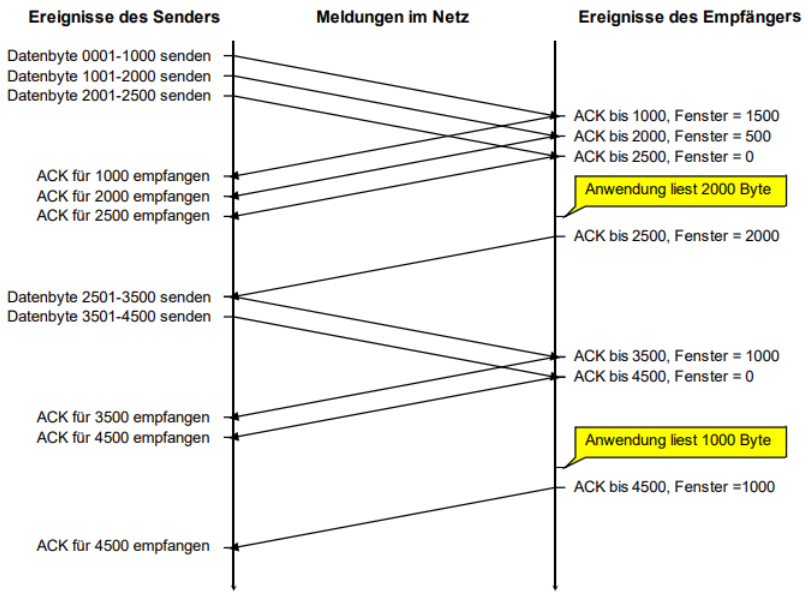
\includegraphics[width=1\linewidth]{images/flusssteuerung_tcp.png}\\
    Annahmen:
    \begin{itemize}
        \item 2'500 Byte Empfangspuffer
        \item 5'000 Bytes Daten
    \end{itemize}
    Ablauf:
    \begin{itemize}
        \item Fenstergrösse des Empfängers wird im WindowFeld des TCP-Headers übermittelt
        \item Wireshark gibt dieses als Advertized Window Size an
        \item Sender-Applikation benötigt nur einen Aufruf von send() für die gesamten 5'000 Bytes
    \end{itemize}
\end{example2}

\begin{formula}{Bandwidth Delay Product (TCP-Puffergrössen)}\\
    Wie gross sollten die Sende- und Empfangsbuffer gewählt werden, um eine TCP-Verbindung nicht auszubremsen?
    $$BDP (bits) = RTT (sec) \cdot Bandbreite (bps)$$
    RTT = Round-Trip-Time\\
    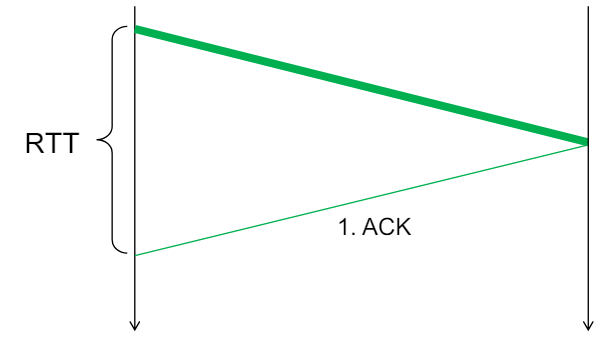
\includegraphics[width=0.5\linewidth]{images/bdp_rtt.png}
\end{formula}

\begin{concept}{Congestion Control}\\
    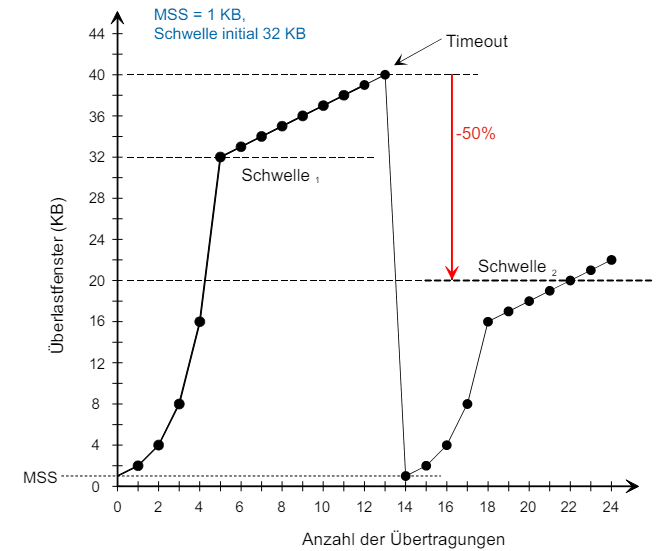
\includegraphics[width=0.75\linewidth]{images/congestion_control.png}\\
    Überlast des Netzes\\
    TCP benutzt den Paketverlust als Masseinheit für Überlastung und reagiert durch Absenken der Übertragungsrate (Slow Start). Dadurch kann die Überlastung überwacht und verhindert werden.\\
    Hierfür pflegt jeder Sender zwei Fenster (vom Sender gewährtes Fenster, Überlastungsfenster). Das Minimum der Fenster stellt die Anzahl Bytes dar, die gesendet werden können.\\
    \textbf{Wichtig:} Der Sender kombiniert das Congestion Window mit den Informationen zur Flow Control vom Empfänger und schickt unbestätigte Daten bis zum Erreichen von: min \{Congestion Window, Advertised Window\}
\end{concept}

\subsection{Zusammenfassung Transport Layer}

\begin{formula}{Vergleich Layer 4 und Layer 2}\\
    Herausforderungen zur Zuverlässigkeit zwischen Ethernet (Schicht 2) und TCP (Schicht 4):
    \begin{itemize}
        \item Spalte 1: Potentielle Probleme / Fehlersituationen
        \item Spalte 2/3: Charakteristika derselben auf Schicht 2 und Schicht 4
        \item Spalte 4: Massnahmen bei TCP, um diese Probleme zu lösen
    \end{itemize}
        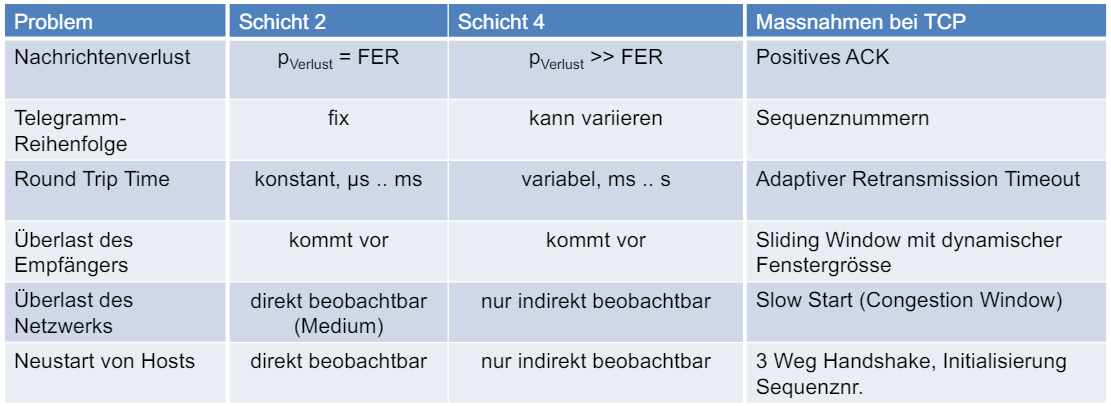
\includegraphics[width=1\linewidth]{vergleich_layer_2_4.png}
\end{formula}

\begin{KR}{Key Takes Transport Layer}
    \begin{itemize}
        \item Die Transportschicht bietet Applikationen einen Ende-zu-Ende Dienst
        \begin{itemize}
            \item Port Nummern bei TCP / UDP werden verwendet um Applikationen zu identifizieren
            \item Server Applikationen warten (=listen) an bekannten (well-known) Ports
            \item Der Vorgang, lokal Daten an verschiedene Instanzen höherer Protokollschichten zu verteilen, wird als Multiplexing / Demultiplexing bezeichnet und findet auf allen Schichten statt
            \begin{itemize}
                \item „Type“ bei Ethernet, „Protocol“ bei IP, „Port“ bei TCP/UDP
            \end{itemize}
        \end{itemize}
        \item UDP gibt die Eigenschaften von IP (verbindungslos, unzuverlässig) praktisch unverändert weiter
        \begin{itemize}
            \item Zusatzfunktionalität: Multiplexen / Demultiplexen aufgrund der Port Nummer und Checksumme über die gesamten Daten (IP schützt nur den Header)
        \end{itemize}
        \item TCP bietet einen verbindungsorientierten, zuverlässigen Dienst
        \begin{itemize}
            \item Für die Applikation sehr ähnlich zum Lesen / Schreiben eines Files
            \item Verbindung von einer Client-Application zu einer Server-Applikation
            \item Verbindungsaufbau wird immer vom Client initialisiert
            \item Nach dem Verbindungsaufbau ist die Kommunikation symmetrisch, beide Kommunikationspartner können das Schliessen der Verbindung initiieren
        \end{itemize}
        \item Ein UDP Datagramm / TCP Segment wird in genau ein IP Paket eingefügt
        \item TCP verwendet folgende Massnahmen, um die sichere Kommunikation zu gewährleisten:
        \begin{itemize}
            \item 32-Bit Sequenznummern – jedes Byte im Datenstrom ist eindeutig identifiziert
            \item 3-Wege Handshake beim Verbindungsaufbau mit zufälliger Initialisierung der Sequenznummern
            \item Kontrollierter Verbindungsabbau mit der Möglichkeit, ausstehende Daten zu senden
            \item Adaptive Timeouts basierend auf Wert und Varianz der gemessenen Round-Trip Zeiten
            \item Schutz des Empfängers vor Überlast durch dynamische Anpassung der Fenstergrösse beim Sliding Window Protokoll (Advertised Window, wird dem Sender vom Empfänger mitgeteilt)
            \item Schutz des Netzwerks vor Überlast durch Congestion Control (im Sender) mit dem Slow Start Algorithmus
        \end{itemize}
    \end{itemize}

\end{KR}
